\documentclass[main.tex]{subfiles}

\begin{document}
\chapter{Контрольная работа №~2}

Цель работы: Изучение основ таймеров, решение различных задач с помощью таймеров. Получение практических навыков по работе с инструментальными средствами отладки микроконтроллеров AVR.

Работа выполняется в среде Atmel Studio.

\section{Теоретические сведения}

Микроконтроллеры AVR семейства Mega в зависимости от модели имеют в своем составе от двух до четырех таймеров/счетчиков общего назначения.

Таймеры ATmega16x:
\begin{itemize}
\item T0 --- 8-разрядный;
\item T1 --- 16-разрядный;
\item T2 --- 8-разрядный.
\end{itemize}

Во всех моделях микроконтроллеров семейства присутствуют, как минимум, два таймера/счетчик~--- T0 и T1. Таймер/счетчик T0 имеет минимальный набор функций, зависящий тем не менее от модели микроконтроллера. В одних моделях он может использоваться только для отсчета и измерения временных интервалов или как счетчик внешних событий. В других моделях к этим функциям добавляется возможность генерации сигналов с широтно-импульсной модуляцией (ШИМ) фиксированной разрядности, а также возможность работать в асинхронном режиме в качестве часов реального времени.

Таймер/счетчик T1 тоже может использоваться для отсчета временных  интервалов и как счетчик внешних событий. Кроме того, он может выполнять запоминание своего состояния по внешнему сигналу. Как и таймер/счетчик T0, он может работать в качестве широтно-импульсного модулятора, но уже переменной разрядности и к тому же многоканального (количество каналов зависит от модели).

Таймер/счетчик T2 полностью аналогичен таймеру/счетчику T0. При наличии в микроконтроллере обоих таймеров/счетчиков, один из них может работать в асинхронном режиме, а другой — в качестве счетчика внешних событий.

Таймер/счетчик T3 по функциональным возможностям идентичен таймеру/счетчику T1.

%В составе всех микроконтроллеров семейства имеется также сторожевой таймер, являющийся непременным атрибутом всех современных микроконтроллеров. Этот таймер позволяет избежать несанкционированного зацикливания программы, возникающего по тем или иным причинам.

Использование альтернативных функций линий портов ввода/вывода ATmega16x (см.~рисунок \ref{fig:pins}):

    \begin{tabular}{|l|l|l|}
    \hline
    Название & Пин & Описание\\
    \hline
    T0 & PB0 & Вход внешнего сигнала таймера T0\\
    OC0 & PB3 & Выход схемы сравнения таймера T0\\
    \hline
    T1 & PB1 & Вход внешнего сигнала таймера T1\\
    ICP & PD6 & Вход захвата таймера T1\\
    OC1A & PD5 & Выход схемы сравнения таймера T1\\
    OC1B & PD4 & Выход схемы сравнения таймера T1\\
    \hline
    OC2 & PD7 & Выход схемы сравнения таймера T2\\
    \hline
    TOSC1 & PC6 & Вход для подключения резонатора\\
    TOSC2 & PC7 & Выход для подключения резонатора\\
    \hline
    \end{tabular}

\begin{figure}[h]
\centering
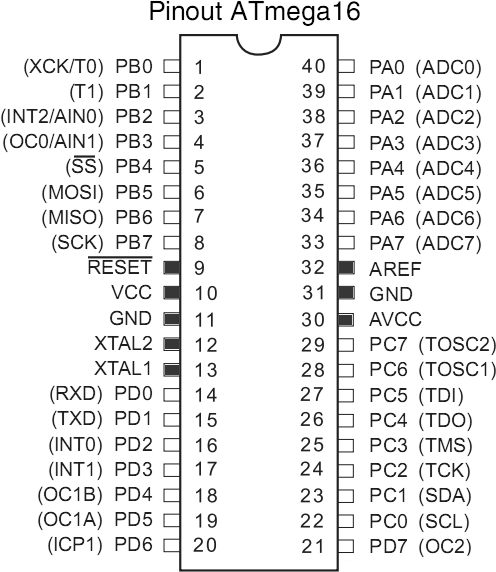
\includegraphics[scale=0.25]{images/3_pins.png}
\caption{Распиновка микроконтроллера ATmega16}
\label{fig:pins}
\end{figure}

\begin{lstlisting}
.include "m16def.inc"  $\color{red}\textrm{; ATmeta16x}$
$\color{red}\textrm{; …}$
    sbi DDRD, DDD7     $\color{red}\textrm{; выход}$

    ldi tmp, 255
    out OCR2, tmp  $\color{red}\textrm{; Timer/Counter2 Output Compare Reg.}$
    $\color{red}\textrm{; Waveform Genration Mode. 10 == режим работы CTC}$
    $\color{red}\textrm{; Compare Output Mode. 01 == переключение выхода}$
    $\color{red}\textrm{;  при совпадении}$
    $\color{red}\textrm{; Clock Select. Предделитель 101 == clk/1024}$
    ldi tmp, (1<<FOC2)|(0<<WGM20)|\
      (0<<COM21)|(1<<COM20)|(1<<WGM21)|\
      (1<<CS22)|(0<<CS21)|(1<<CS20)
    out TCCR2, tmp  $\color{red}\textrm{; Timer/Counter2 Control Register}$
$\color{red}\textrm{; …}$
\end{lstlisting}










\newpage
\section{Варианты заданий}\label{ch:var2}

Задание на контрольную работу: необходимо организовать устройство для отображения информации на семисегментном светодиодном индикаторе. Информация на индикаторе меняется от нажатия клавиш.

При выполнении контрольной работы, обратите внимание на раздел <<\nameref{ch:str}>> (стр.~\pageref{ch:str}).

\begin{small}
\vspace{12px}
\noindent
\begin{tabularx}{\textwidth}{|X|}
\hline
\textbf{Вариант 1}\\
\hline
Мигать одним светодиодом с частотой 1 ГЦ, вторым~--- с частотой 2 Гц.\\
\hline
\end{tabularx}

\vspace{12px}
\noindent
\begin{tabularx}{\textwidth}{|X|}
\hline
\textbf{Вариант 2}\\
\hline
Считать количество входных импульсов за 1 секунду.\\
\hline
\end{tabularx}

\vspace{12px}
\noindent
\begin{tabularx}{\textwidth}{|X|}
\hline
\textbf{Вариант 3}\\
\hline
Мигать одним светодиодом, по нажатию одной клавиши увеличивать частоту в два раза, при нажатии другой~--- уменьшать в два раза.\\
\hline
\end{tabularx}

\vspace{12px}
\noindent
\begin{tabularx}{\textwidth}{|X|}
\hline
\textbf{Вариант 4}\\
\hline
Посчитать количество нажатий клавиши за 10 секунд.\\
\hline
\end{tabularx}

\vspace{12px}
\noindent
\begin{tabularx}{\textwidth}{|X|}
\hline
\textbf{Вариант 5}\\
\hline
Двоичный секундомер, при нажатии одной клавиши увеличивать частоту отсчёта, при нажатии другой~--- уменьшать.\\
\hline
\end{tabularx}

\vspace{12px}
\noindent
\begin{tabularx}{\textwidth}{|X|}
\hline
\textbf{Вариант 6}\\
\hline
Клавишами установить частоту, запустить таймер с соответствующей индикацией.\\
\hline
\end{tabularx}

\vspace{12px}
\noindent
\begin{tabularx}{\textwidth}{|X|}
\hline
\textbf{Вариант 7}\\
\hline
С четырехсекундной задержкой после нажатия клавиши запустить таймер с соответствующей индикацией.\\
\hline
\end{tabularx}

\vspace{12px}
\noindent
\begin{tabularx}{\textwidth}{|X|}
\hline
\textbf{Вариант 8}\\
\hline
С трехсекундной задержкой после нажатия клавиши остановить таймер с соответствующей индикацией.\\
\hline
\end{tabularx}

\vspace{12px}
\noindent
\begin{tabularx}{\textwidth}{|X|}
\hline
\textbf{Вариант 9}\\
\hline
Одна октава на звукомоделирующем пьезоэлементе.\\
\hline
\end{tabularx}

\vspace{12px}
\noindent
\begin{tabularx}{\textwidth}{|X|}
\hline
\textbf{Вариант 10}\\
\hline
Секундомер, первая клавиша~--- запуск, вторая~--- останов, третья~--- сброс.\\
\hline
\end{tabularx}

\vspace{12px}
\noindent
\begin{tabularx}{\textwidth}{|X|}
\hline
\textbf{Вариант 11}\\
\hline
По нажатию клавиши зажечь светодиод с помощью ШИМ.\\
\hline
\end{tabularx}

\vspace{12px}
\noindent
\begin{tabularx}{\textwidth}{|X|}
\hline
\textbf{Вариант 12}\\
\hline
Одной клавишей уменьшать яркость светодиода, другой~--- увеличивать (ШИМ).\\
\hline
\end{tabularx}

\vspace{12px}
\noindent
\begin{tabularx}{\textwidth}{|X|}
\hline
\textbf{Вариант 13}\\
\hline
Одновременно зажигать один светодиод и гасить дугой (ШИМ).\\
\hline
\end{tabularx}

\vspace{12px}
\noindent
\begin{tabularx}{\textwidth}{|X|}
\hline
\textbf{Вариант 14}\\
\hline
Последовательно зажечь все 8 светодиодов (ШИМ).\\
\hline
\end{tabularx}
\end{small}

\end{document}
